\documentclass[a4paper]{article}
\usepackage{interspeech2012,amssymb,amsmath,graphicx}

\sloppy	% better line breaks
%\ninept	% optional

\title{Student Response Analysis using Textual Entailment}

%%%%%%%%%%%%%%%%%%%%%%%%%%%%%%%%%%%%%%%%
%% If multiple authors, uncomment and edit the lines shown below.       %%
%% Note that each line must be emphasized {\em } by itself.                  %%
%% (by Stephen Martucci, author of spconf.sty).                                     %%
%%%%%%%%%%%%%%%%%%%%%%%%%%%%%%%%%%%%%%%%
%\makeatletter
%\def\name#1{\gdef\@name{#1\\}}
%\makeatother
%\name{{\em Firstname1 Lastname1, Firstname2 Lastname2, Firstname3 Lastname3,}\\
%      {\em Firstname4 Lastname4, Firstname5 Lastname5, Firstname6 Lastname6,
%      Firstname7 Lastname7}}
% End of required multiple authors changes %%%%%%%%%%%%%%%%%

\makeatletter
\def\name#1{\gdef\@name{#1\\}}
\makeatother
\name{{\bf Ashudeep Singh$^1$, Devanshu Arya$^2$, Amitabha Mukerjee$^1$}}

\address{$^1$Computer Science and Engineering, Indian Institute of Technology Kanpur \\
               $^2$Electrical Engineering, Indian Institute of Technology Kanpur \\
{\small \tt ashudeep@iitk.ac.in, devanshu@iitk.ac.in, amit@cse.iitk.ac.in}}

%\twoauthors{Karen Sp\"{a}rck Jones.}{Department of Speech and Hearing \\
%  Brittania University, Ambridge, Voiceland \\
%  {\small \tt Karen@sh.brittania.edu} }
%  {Rose Tyler}{Department of Linguistics \\
%  University of Speechcity, Speechland \\
%  {\small \tt RTyler@ling.speech.edu} }

\begin{document}
\maketitle
\vspace{-1.5cm}
\section{Introduction}
A major task in Educational NLP is to assess student responses to examination questions, homeworks and intelligent tutors. Much of the related work has been done in evaluating student essays \cite{attali}\cite{shermi}, error detection and correction \cite{leacock} and grade level text classification \cite{peterson}. A subtask in student dialogue systems is Student Response Analysis (SRA) i.e. given a question and a few reference answers, the system needs to analyze student response and decide whether it is correct or else give a suitable feedback. A key requirement to accomplish this is semantic inference, for example to detect whether the student answers say the same thing as the reference answer in different words or contradict it.
\section{Recognizing Textual Entailment}
Recognizing Textual Entailment (RTE 2005-2012) is a series of challenges where many systems that can recognize semantic inference have been presented. This task, as a part of SemEval 2013, was aimed at bringing Educational NLP closer to semantic inference community.   
\section{Student Response Analysis Corpus}
The corpus contains manually labeled students responses to explanation and definition questions\cite{dk}. Specifically, the data set contains a question, a reference answer and a 1-2 sentence student answer. Each student answer is labeled as one of the five judgments by a human annotator:
\begin{itemize}
	\item \textbf{Correct}, when the student answer is a complete and correct representation of one of the reference answers.
	\item \textbf{Partially correct but Incomplete}, when the student answer is correct to the extent it is written, but is not complete.
	\item \textbf{Contradictory}, when the student answer contradicts the reference answer, i.e. both cannot be correct at the same time.
	\item \textbf{Irrelevant}, when the student answer is irrelevant to the reference answer although it may still be talking about the reference answer. 
	\item \textbf{Non-Domain}, when the student answer lacks domain content, i.e. the student may be asking for `help', `advice' etc. like `I don't know', `what the book says', `you are stupid'.\\
\end{itemize}
The SRA Corpus consists of 2 subsets: \textsc{Beetle} and \textsc{SciEntsBank}. The \textsc{Beetle} corpus contains 56 questions in basic electricity and electronics domain with 3000 student answers. The \textsc{SciEntsBank} corpus\cite{nlsn} contains 197 assessment questions with 10,000 student answers in 15 different science domains.

\section{Main Task}
The main task is to produce an assessment of student answers to explanation and definition questions asked seen in practice exercises, tests or dialogue. The main task is to assess a student's answer at 3 different levels of granularity, namely:
\begin{itemize}
	\item \textbf{5-way task} 
	\begin{itemize}
	\item correct
	\item partially correct but incomplete
	\item contradictory
	\item irrelevant
	\item not-in-the-domain
	\end{itemize}
	\item \textbf{3-way task}
	\begin{itemize}
	\item correct
	\item contradictory
	\item incorrect : comprising of paritally-correct incomplete, irrelevant and non-domain answers.
	\end{itemize}
	\item \textbf{2-way task}
	\begin{itemize}
	\item correct
	\item incorrect
	\end{itemize}
\end{itemize} 

Such recognition of partial entailment may have various utilities in the educational setting based on identifying the missing parts in the student answer, and may similarly have value in other applications such as summarization or question answering.

\section{Approach}
\begin{figure}[htb]
\begin{minipage}[b]{1.1\linewidth}
  \centering
  \centerline{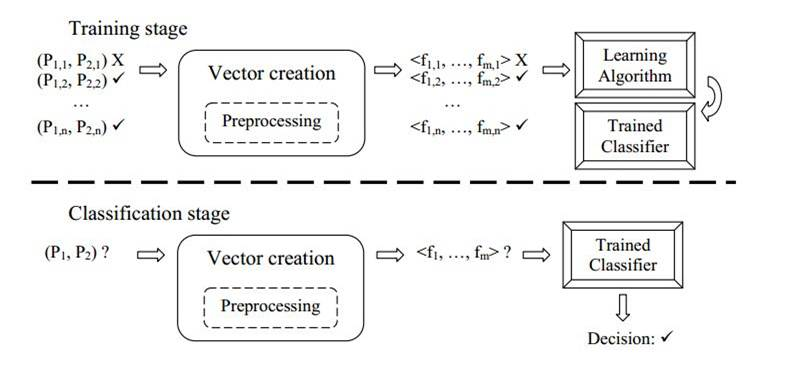
\includegraphics[width=9cm,height=3.0cm]{Picture1.jpg}}
  \vspace{-0.8cm}
  \centerline{}\medskip
\end{minipage}
\caption{Figure \cite {pic} showing in brief the process of Textual Entailment Recognition via supervised machine learning}
\label{fig1}
\end{figure}
There is a correlation between textual entailment and answer correctness. In a typical answer assessment scenario, we expect a correct answer to entail the reference answer. However a student may wish to skip the details already mentioned in the question. So the problem basically is whether the answer, along with the question entails the reference answer. 
Let the question be $q$, student answer be $s$ and the reference answer be $r$. Correctness means $a \wedge s\Rightarrow r$ and Contradiction means $s \wedge\Rightarrow \neg r$.

 \textit{Recognizing textual entailment} challenges have addressed such challenges since 2005\cite{rte}. We plan to use a RTE system along with shallow text features to train on the SRA (\textsc{Beetle} and \textsc{SciEntsBank}) dataset and testing it on the test dataset provided. The evaluation metrics used will be according to the SemEval 2013, Task 7 problem statement, which are intuitively based on the $precision$ and $recall$ values for each class. The two important measures that describe the systems performance here are:
\begin{itemize}
	\item \textbf{Macro-Average}: The average of the F1-scores of all the classes.
	\item \textbf{Micro-Average}: The weighted average of all the classes, where weights are the frequencies of each class in the test set.
\end{itemize}

\section{Train and Test Scenarios}
The dataset was used to create two scenarios for traing and testin purposes, namely Unseen Answers(UA) and Unseen Questios(UQ). 
\begin{itemize}
	\item In \textbf{Unseen Answers} case,
all student answered to 1 to 2 randomly selected questions from each of the modules forming the training set whuch was held out as the test data set.
The objective for creating such dataset was to test the system performance on new questions within the same set of domains.
\item In \textbf{Unseen Questions} case, 4 randomly selected student answers to each of the questions in the training set was withheld. This would serve as test data for system performance on the 
same questions as contained in the training set. 
\end{itemize} 
 
\section{Features}
To build a system that evaluates student answers, we use the labeled training set to train our system on. For this, we require numerous text-similarity and overlap features that can well describe how close the students answer is to the reference answer. In the further sub-sections we describe the features that defined our feature-set on which the system was trained.
\subsection{Baseline Features}
It includes all of the features provided by the task organizers as baseline. There are four types of lexically-driven text similarity measures, and each is computed by comparing the learner response to both the expected answer(s) and the question, resulting in eight features in total -- four in comparison the question, four with the maximum overlapping reference answer. The four types of measures include:
\begin{itemize}
	\item \textbf{Overlapping Words} : It is simply the number of overlapping words between the student and reference answers.
	\item \textbf{Cosine Similarity} : Representing each answer as a bag-of-words vector, cosine similarity is the cosine of the angle between the vectors.
	\item \textbf{F1 Score} : Defining precision and recall on the number of hits i.e. co-occurences of words, F1-score is the harmonic mean of these precision, recall values.
	\item \textbf{Lesk Score} : Simplified lesk score is used to compare the overlap in meanings of the words in answers. \cite{banerjee}
\end{itemize}

Following are the features we added to the system to make it perform better:\\
\subsection{Matching Content words}We created a vocabulary of content words i.e. the words dealing with the subject talked about in the question-answering assignment. As the data-set was from electronics and electrical domain question-answers, we used a hand-made dictionary of such words.

\subsection{Polarity} 
Our training feature set includes a polarity feature that captures the presence (or absence) of linguistic markers of negative polarity in both text and hypothesis, such as not, no, few, without, except etc.. If there is simultaneous existence or non-existence of a negative polarity word in both the students answers and the reference answers or the question, the polarity feature contained a value of 1 otherwise a negative value was assigned.
\subsection{Antonymy}
This feature checks whether an aligned pair of words in respective answers and questions appear to be antonymous by consulting WordNet ontology\cite{wordnet}. If there is an occurrence of such pair of antonym words, then it checks the polarity of the word preceding these words. For example, if there are words in the text and hypothesis as good and bad than it assigns a boolean positive  to this feature. However, if $bad$ is preceeded by $not$, than this feature returns a boolean negative. 
\subsection{Synonymy}
Similar to antonymy features, this feature checks for the presence of synonym words in the texts and then checks the polarity of the preceding word. The assignment of boolean digits is done in the same way as in Antonym Features.
\subsection{Number, Date and Time Features}
These features recognize (mis-)matches between numbers, dates, and times, between the texts. If the numerical data in both the text lies in the same range than it is assigned a positive boolean otherwise a negative value is given.
\subsection{Wu-Palmer Similarity}
For each word in the student's answer we add the highest Wu-Palmer similarity with a word from the reference answer. Wu-Palmer similarity is a measure that uses WordNet ontology to say how similar two words are.\cite{wup} \\

$ \frac{2 . depth(lcs)}{depth(s_1) + depth(s_2)}$, where $lcs$ is the least common subsequence, $s_1$ and $s_2$ are the strings.
\section{Results}
We ran our system on the test-sets according to the two scenarios -- \textbf{UA} (Unseen Answers) and \textbf{UQ} (Unseen Questions). We incrementally added features to our system and observed the Micro and Macro-average of the F1-scores. Following are the results of our system compared with the Baseline and top 3 entries of each task:\\ 
The features have been represented as abbreviations:
\begin{itemize}
	\item \textbf{CW} -- Matching Content Words
	\item \textbf{P} -- Polarity feature
	\item \textbf{S} -- Synonymy feature
	\item \textbf{A} -- Anonymy feature
	\item \textbf{N} -- Number, date and Time features
	\item \textbf{WuP} -- Wu-Palmer similarity
\end{itemize}
The classifiers used are: 
\begin{itemize}
	\item \textbf{j48} -- Weka implementation of Decision Trees
	\item \textbf{k-NN} -- k-Nearest Neighbors using k=35.
\end{itemize}
\begin{table}[htb!]
\eightpt
\setlength{\tabcolsep}{4pt}



\begin{tabular}{|l|l|l|l|l|l|}
\hline
\textbf{Features}& \multirow{Classifier} & \multicolumn{2}{|c|}{UA} & \multicolumn{2}{|c|}{UQ} \\ \cline{3-6}

                                                             &            & Macro      & Micro     & Macro      & Micro     \\ \hline
 \textbf{Baseline}& j48        & 0.42       & 0.48      & 0.41       & 0.46      \\\hline

\multirow{\textbf{Baseline+CW}}             & j48        & 0.46       & 0.53      & 0.39       & 0.45      \\\hline
 & Logistic   & 0.45       & 0.54      & 0.43       & 0.51      \\\hline
																														
 \textbf{Baseline+CW+P+N }     & j48        & 0.49       & 0.57      & 0.50       & 0.51      \\\hline
{\multirow{\textbf{Baseline+CW+P+N+S+A+WuP}}} & j48        & 0.47       & 0.57      & 0.49       & 0.5       \\\hline
 & K-NN       & 0.50       & 0.61      & 0.47       & 0.51 \\ \hline
\textbf{ETS$_2$} & j48        & 0.619       & 0.705      & 0.552       & 0.614       \\
\textbf{CoMeT$_1$}& - & 0.569 & 0.675 & 0.300 &0.445\\
\textbf{EHUALM$_1$}&-&0.526&0.566&0.300&0.416\\\hline
\end{tabular}
\caption{Comparison of our system's results with the top-3 entries in the SemEval 2013 5-way task}
\end{table}


\begin{table}[htb!]
\eightpt
\setlength{\tabcolsep}{4pt}
\begin{tabular}{|l|l|l|l|l|l|}
\hline
\multirow{ \textbf{Features}}                & \multirow{Classifier} & \multicolumn{2}{|c|}{UA} & \multicolumn{2}{|c|}{UA} \\ \cline{3-6} 
 &         & Macro       & Micro      & Macro       & Micro      \\ \hline
 \textbf{Baseline}             & j48     & 0.55        & 0.58       & 0.48        & 0.50       \\ \hline
\multirow{ \textbf{Baseline+CW+P+N+S+A+WuP}} & j48     & 0.57        & 0.60       & 0.46        & 0.48       \\ \cline{2-6} 
 & KNN     & 0.63        & 0.65       & 0.49        & 0.51       \\ \hline
\textbf{ETS$_2$\footnote{Education Testing Services, NJ, USA}\cite{heilman}} & j48        & 0.71       & 0.723      & 0.585       & 0.597       \\
\textbf{CoMeT$_1$}& - & 0.715 & 0.728 & 0.466 &0.488\\
\textbf{ETS$_1$}&j48&0.592&0.619&0.521&0.512\\\hline
\end{tabular}

\caption{Comparison of our system's results with the top-3 entries in the SemEval 2013 3-way task}
\end{table}





\begin{table}[htb!]
\eightpt
\setlength{\tabcolsep}{4pt}
\begin{tabular}{|l|l|l|l|l|l|}
\hline
\multirow{ \textbf{Features}}                    & \multirow{Classifier} & \multicolumn{2}{|c|}{UA} & \multicolumn{2}{|c|}{UQ} \\ \cline{3-6} 
     &            & Macro       & Micro      & Macro       & Micro      \\ \hline
 \textbf{Baseline}                 & j48        & 0.78        & 0.80       & 0.73        & 0.73       \\ \hline
 \textbf{Baseline+CW+P+N}  & j48        & 0.76        & 0.77       & 0.7         & 0.71       \\ \hline
\multirow{ \textbf{Baseline+CW+P+N+S+A+WuP}}& j48        & 0.77        & 0.77       & 0.72        & 0.73       \\ \cline{2-6} 
     & K-NN       & 0.81        & 0.82       & 0.73        & 0.74       \\ \hline
		\textbf{ETS$_2$} & j48        & 0.833       &-      & 0.702       &-       \\
\textbf{CoMeT$_1$}&- & 0.833 & -& 0.695 &-\\
\textbf{CU$_1$}&-&0.778&-&0.689&-\\\hline
\end{tabular}
\caption{Comparison of our system's results with the top-3 entries in the SemEval 2013 5-way task}

\end{table}


\section{Conclusion}
The recognition of textual entailment in text has been hot for a few years now and its application in Student Response Analysis looks promising. We presented our feature set that we used to define our systems training parameters. The results reflect the system's ability to correctly evaluate student answers in majority cases. But its quite sure that there is a long way to go before we can develop robust systems that do the task in everyday classroom scenario.





\eightpt
\bibliographystyle{IEEEtran}
\begin{thebibliography}{10}
\bibitem{attali}
Yigal Attali and Jill Burstein. 2006.\textit{ Automated essay
scoring with e-rater v.2}. The Journal of Technology,
Learning, and Assessment, 4\(3\), February.
\bibitem{shermi}
Mark D. Shermis and Jill Burstein, editors. 2013. \textit{Handbook
on Automated Essay Evaluation: Current Applications
and New Directions.} Routledge
\bibitem{peterson}
Sarah Petersen and Mari Ostendorf. 2009. \textit{A machine
learning approach to reading level assessment.} Computer,
Speech and Language, 23\(1\):89ֱ06.
\bibitem{leacock}
Claudia Leacock, Martin Chodorow, Michael Gamon,
and Joel R. Tetreault. 2010. \textit{Automated Grammatical
Error Detection for Language Learners}. Synthesis
Lectures on Human Language Technologies. Morgan
\& Claypool Publishers.
\bibitem{rte}
Dagan, I., Glickman, O., \& Magnini, B. \(2006\). \textit{The pascal recognising textual entailment challenge.} In Machine Learning Challenges. Evaluating Predictive Uncertainty, Visual Object Classification, and Recognising Tectual Entailment \(pp. 177-190\). Springer Berlin Heidelberg.
\bibitem{nlsn}Rodney D. Nielsen, Wayne Ward, James H. Martin, and
Martha Palmer. 2008b.\textit{ Annotating studentsҠunderstanding
of science concepts.} In Proceedings of the
Sixth International Language Resources and Evaluation
Conference, \(LREC08\), Marrakech, Morocco. 
\bibitem{pic}
Androutsopoulos, Ion, and Prodromos Malakasiotis. "A survey of paraphrasing and textual entailment methods." arXiv preprint arXiv:0912.3747 (2009).
\bibitem{dk}
Myroslava O. Dzikovska, Rodney D. Nielsen, and Chris
Brew. 2012. \textit{Towards effective tutorial feedback for
explanation questions: A dataset and baselines.} In
Proc. of 2012 Conference of NAACL: Human Language
Technologies, pages 200ֲ10.
\bibitem{banerjee} Banerjee, S., \& Pedersen, T. (2002). \textit{An adapted Lesk algorithm for word sense disambiguation using WordNet. In Computational linguistics and intelligent text processing (pp. 136-145).} Springer Berlin Heidelberg.
\bibitem{heilman}  Heilman, M., \& Madnani, N. \texit{ETS: Domain Adaptation and Stacking for Short Answer Scoring.} SemEval 2013.
\bibitem{wup} Pedersen, T., Patwardhan, S., \& Michelizzi, J. (2004, May). WordNet:: Similarity: measuring the relatedness of concepts. In Demonstration Papers at HLT-NAACL 2004 (pp. 38-41). Association for Computational Linguistics.
\bibitem{wordnet} Miller, G. A. (1995). WordNet: a lexical database for English. Communications of the ACM, 38(11), 39-41.
\end{thebibliography}
\end{document}